\documentclass[11pt,letterpaper]{article}

% ── Packages ──────────────────────────────────────────────────────────────────
\usepackage[margin=1in]{geometry}
\usepackage{amsmath,amssymb,amsfonts}
\usepackage{graphicx}
\usepackage[numbers,sort&compress]{natbib}
\usepackage{hyperref}
\usepackage{booktabs}
\usepackage{xcolor}
\usepackage{microtype}
\usepackage{float}
\usepackage{caption}
\usepackage{subcaption}
\usepackage{setspace}
\usepackage{authblk}

\hypersetup{colorlinks=true, linkcolor=blue!60!black, citecolor=blue!60!black, urlcolor=blue!60!black}
\captionsetup{font=small, labelfont=bf}
\onehalfspacing

% ── Math shortcuts ────────────────────────────────────────────────────────────
\newcommand{\GP}{\mathcal{GP}}
\newcommand{\KL}{\mathrm{KL}}
\newcommand{\E}{\mathbb{E}}
\newcommand{\R}{\mathbb{R}}
\newcommand{\bx}{\mathbf{x}}
\newcommand{\bZ}{\mathbf{Z}}
\newcommand{\bu}{\mathbf{u}}
\newcommand{\bm}{\mathbf{m}}

% ══════════════════════════════════════════════════════════════════════════════
\title{\textbf{Working Memory as Dynamic Bayesian Inference\\over Continuous Feature Space}}

\author[1]{Dongyu Gong (dongyu.gong@yale.edu)}
\author[1]{Mario Belledonne (mario.belledonne@yale.edu)}
\author[1,2]{Ilker Yildirim (ilker.yildirim@yale.edu)}
\affil[1]{Department of Psychology, Yale University}
\affil[2]{Wu Tsai Institute, Yale University}

\date{}

\begin{document}
\maketitle

% ╔═══════════════════════════════════════════════════════════════════════════╗
% ║  ABSTRACT                                                                 ║
% ╚═══════════════════════════════════════════════════════════════════════════╝
\begin{abstract}
Visual working memory (VWM) supports the short-term retention of a small number of visual items, yet the computational principles governing how items are encoded, actively maintained, and later retrieved remain debated. Existing models characterize VWM as either discrete slots or divisible resources, but neither provides a unified, algorithmic-level account of the full range of behavioral phenomena. Here we introduce MemGP, a framework that reconceptualizes VWM as dynamic Bayesian inference over a continuous function on circular location--feature space, implemented via sparse variational Gaussian processes. Encoding corresponds to fitting a GP posterior to noisy sensory observations; maintenance operates through self-rehearsal against a forgetting pressure (KL divergence toward the prior), with goal-directed attention reweighting the variational objective; and retrieval evaluates the posterior at the probed location. Without ad hoc mechanisms, this single framework quantitatively reproduces set-size--dependent precision loss, apparent guessing behavior, retrocue benefits that scale with memory load, cue-timing sensitivity, flexible resource reallocation across sequential cues, and encoding-time--dependent repulsion bias---phenomena that previously required separate models. Formal model comparison confirms that MemGP's emergent error statistics match or surpass leading resource models (IL, EP, SA, VP). These results demonstrate that the core signatures of VWM capacity, precision, and attentional control emerge naturally from a single Bayesian inference process operating over a shared representational substrate.
\end{abstract}

% ╔═══════════════════════════════════════════════════════════════════════════╗
% ║  INTRODUCTION                                                             ║
% ╚═══════════════════════════════════════════════════════════════════════════╝
\section{Introduction}

Visual working memory (VWM) enables the temporary storage and manipulation of visual information to guide ongoing behavior. Despite decades of research, fundamental questions remain about the computational architecture underlying this capacity-limited system. Two dominant theoretical traditions have shaped the field. \emph{Slot-based} models propose that VWM consists of a small, fixed number of discrete memory slots, each storing one item with fixed precision; items exceeding this capacity are simply lost \cite{luckCapacityVisualWorking1997c, zhangDiscreteFixedresolutionRepresentations2008b}. \emph{Resource-based} models, by contrast, propose that a continuous pool of representational resources is distributed across all items, with precision declining as load increases \cite{baysPrecisionVisualWorking2009b, maChangingConceptsWorking2014a, vandenbergVariabilityEncodingPrecision2012}. The most sophisticated resource account, the \emph{Variable-Precision} (VP) model \cite{vandenbergVariabilityEncodingPrecision2012}, further posits that encoding precision fluctuates from trial to trial according to a stochastic distribution (typically Gamma), capturing not only mean precision loss but also the heavy-tailed error distributions observed at high loads.

A third, more mechanistically grounded tradition derives VWM behavior from \emph{neural population coding}. In these models, stimuli are represented by the spiking activity of tuned neural populations, and recall errors arise from probabilistic decoding of noisy population responses \cite{baysNoiseNeuralPopulations2014a}. This framework has been extended to account for feature binding through conjunction-selective populations \cite{schneegansNeuralArchitectureFeature2017c}, retrospective attention via gain modulation of population firing rates \cite{baysNeuralModelRetrospective2018a}, and stimulus-specific biases through efficient coding of tuning functions \cite{taylorEfficientCodingVisual2018}. Schneegans et al.\ \cite{schneegansStochasticSamplingProvides2020} showed that VP, Slots-plus-Averaging, and population coding models can all be expressed within a common sampling framework, suggesting that these accounts may be closer than previously thought.

Despite this convergence, no existing framework---whether descriptive or neural---provides a complete, algorithmic-level account of how memory representations are formed, actively maintained over time, and read out at test. Slot and resource models are fundamentally \emph{descriptive}: they specify the statistical structure of errors at retrieval but not the algorithmic operations that produce those errors. Slot models cannot explain the continuous decline in precision with set size or the systematic inter-item interference effects observed in recall \cite{baysPrecisionVisualWorking2009b, chunharasAdaptivePerspectiveVisual2022a}. Resource models, including VP, offer more flexible accounts of precision but typically lack an explicit mechanism for how attention dynamically redistributes resources during maintenance---a phenomenon robustly demonstrated by retrocue paradigms \cite{souzaRetrocuesRetroactiveAttentional2016, griffinSpeedTime2013, gunseliSerialOffloadingWorking2015}. Neural population models provide the strongest mechanistic grounding, but have not yet been unified into a single framework that simultaneously accounts for set-size effects, dynamic attentional reallocation (retrocueing, cue timing, cue flexibility), and encoding-dependent inter-item biases within a shared computational architecture.

Recent benchmarking efforts have catalogued a rich set of phenomena that any comprehensive model of VWM must explain \cite{oberauerBenchmarksModelsShortterm2018, awhWorkingMemoryNeeds2025, baysRepresentationComputationVisual2024}: (a) set-size--dependent precision loss and apparent guessing, (b) retrocue benefits that scale with memory load, (c) flexible reallocation of the retrocue benefit between items within a trial, (d) cue-timing effects, and (e) systematic, distance-dependent inter-item repulsion bias that interacts with encoding duration \cite{chunharasAdaptivePerspectiveVisual2022a}. No existing model accounts for all of these phenomena within a single, unified framework.

Here we propose \textbf{MemGP}, a computational framework that reconceptualizes VWM as dynamic Bayesian inference over a continuous two-dimensional function defined on circular location $\times$ feature (color) space. Like neural population models, MemGP derives behavioral phenomena from a shared representational substrate rather than fitting error distributions post hoc; unlike them, it operates at the level of continuous function-space inference, providing explicit computational accounts of encoding, goal-directed maintenance, and retrieval within a single variational objective. The computational substrate is a \emph{sparse variational Gaussian process} (SVGP) \cite{tiaoHandbookSparseVariational2019, leibfriedTutorialSparseGaussian2022}, chosen for three key properties. First, the GP provides a principled nonparametric prior over smooth functions on the stimulus torus, naturally capturing the circular geometry of both spatial location and color. Second, the sparse inducing-point approximation introduces a finite-capacity bottleneck---analogous to limited neural resources---whose size governs the model's representational capacity. Third, the variational inference framework provides a natural currency for dynamic resource allocation: attention is implemented as differential weighting of the evidence lower bound (ELBO) during maintenance, directly modulating which regions of feature space receive greater computational investment.

The MemGP framework decomposes a memory trial into three computationally explicit stages. \emph{Encoding} corresponds to fitting the GP posterior to noisy, weighted sensory observations. \emph{Maintenance} implements self-rehearsal---the posterior's own predictions serve as targets for continued optimization---with a KL divergence term toward the prior that implements forgetting pressure, and optional attentional gain that reshapes the objective to prioritize cued items. \emph{Retrieval} evaluates the posterior mean along the color dimension at the probed spatial location, optionally with divisive normalization at readout.

We demonstrate that this single framework, with a shared set of approximately ten parameters, quantitatively reproduces all seven classes of phenomena enumerated above. Formal information-theoretic model comparison (AIC, BIC) applied to the error distributions shows that MemGP's emergent mixture statistics align with or surpass predictions from four leading resource models \cite{vandenbergVariabilityEncodingPrecision2012}. Critically, MemGP achieves this not by fitting separate models to each phenomenon, but as \emph{emergent consequences} of a single Bayesian inference process---suggesting that the apparent slots-versus-resources dichotomy dissolves when VWM is understood as continuous function-space inference.

% ╔═══════════════════════════════════════════════════════════════════════════╗
% ║  RESULTS                                                                  ║
% ╚═══════════════════════════════════════════════════════════════════════════╝
\section{Results}

\subsection{The MemGP framework}

MemGP models visual working memory as inference over a latent function $f: [-180, 180)^2 \to \R$ defined on a circular location--color torus (Fig.~\ref{fig:schematic}A). The function's value at a point $(\ell, c)$ represents the memory system's belief that an item with color $c$ was presented at location $\ell$. We place a Gaussian process prior over $f$ with a product of periodic kernels matching the circular geometry of each dimension:
\begin{equation}
    f \sim \GP\bigl(m(\bx),\; \sigma^2 k_{\mathrm{per}}(\ell, \ell'; \lambda_\ell) \cdot k_{\mathrm{per}}(c, c'; \lambda_c)\bigr)
    \label{eq:prior}
\end{equation}
where $k_{\mathrm{per}}$ denotes the periodic kernel with period $360^\circ$, and $\lambda_\ell, \lambda_c$ are lengthscale hyperparameters.

To enable tractable inference with a capacity bottleneck, we employ a sparse variational approximation with $M$ inducing points $\bZ = \{(\ell_m, c_m)\}_{m=1}^M$ arranged on a regular grid over the torus (Fig.~\ref{fig:schematic}D). The variational posterior $q(\bu) = \mathcal{N}(\bm, \mathbf{S})$ over inducing function values $\bu = f(\bZ)$ defines the full approximate posterior via the standard SVGP conditional \cite{tiaoHandbookSparseVariational2019}. The finite size of $M$ naturally limits representational capacity.

\textbf{Encoding.} On each trial, the stimulus array of $N$ items $\{(\ell_i, c_i)\}_{i=1}^N$ generates a cloud of noisy, weighted observations (Fig.~\ref{fig:schematic}A). The model maximizes the variational evidence lower bound (ELBO):
\begin{equation}
    \mathcal{L}_{\mathrm{enc}} = \E_{q(f)}\!\left[\sum_i w_i \log p(y_i \mid f(\bx_i))\right] - \KL\bigl(q(\bu) \,\|\, p(\bu)\bigr)
    \label{eq:elbo_enc}
\end{equation}
where $w_i$ are Gaussian importance weights reflecting the reliability of each observation, and the KL term regularizes toward the prior.

\textbf{Maintenance.} Following encoding, the posterior's own predictions on a dense grid serve as self-rehearsal targets $\tilde{y}_g = \E_{q(f)}[f(\bx_g)]$, frozen at the end of encoding. The maintenance objective is:
\begin{equation}
    \mathcal{L}_{\mathrm{maint}} = -\frac{1}{|\mathcal{G}|}\sum_{g \in \mathcal{G}} a_g \, \E_q\!\left[\log p(\tilde{y}_g \mid f(\bx_g))\right] + \beta \, \KL\bigl(q(\bu) \,\|\, p(\bu)\bigr)
    \label{eq:elbo_maint}
\end{equation}
where $\beta$ controls the rate of forgetting (drift toward the uninformative prior), and $a_g$ are spatial attention weights. When a retrocue indicates item $j$, attention follows a Gaussian gain model (Fig.~\ref{fig:schematic}C):
\begin{equation}
    a(\ell) = 1 + (G - 1)\exp\!\left(-\frac{d(\ell, \ell_j)^2}{2\sigma_s^2}\right)
    \label{eq:attention}
\end{equation}
where $G$ is the peak gain and $d(\cdot, \cdot)$ is circular distance. Absent a cue, all weights equal 1.

\textbf{Retrieval.} At test, the recalled color is the posterior mean's argmax along the color axis at the probed location: $\hat{c} = \arg\max_c \, \mu(\ell_{\mathrm{probe}}, c)$.


% ── Set-size effects ──────────────────────────────────────────────────────
\subsection{Set-size effects emerge from shared representational capacity}

We simulated 100 trials at each set size $N \in \{1, 2, 4, 6\}$ and measured signed recall errors ($N \times 100$ observations per condition). As set size increased, mean absolute error (MAE) rose monotonically from $7.3^\circ$ ($N\!=\!1$) to $38.4^\circ$ ($N\!=\!6$), and the signed-error distribution broadened and developed heavier tails characteristic of increasing uniform-component (``guess'') contributions (Fig.~\ref{fig:setsize}A--B).

To place these results in the context of the resource-model literature, we fit uniform--Von~Mises mixture distributions \cite{zhangDiscreteFixedresolutionRepresentations2008b} to the pooled errors at each set size and compared the resulting mixture weight $w$ and circular standard deviation (CSD) against predictions from four benchmark models: Item-Limit (IL), Slots-plus-Averaging (SA), Equal-Precision (EP), and Variable-Precision (VP) \cite{vandenbergVariabilityEncodingPrecision2012} (Fig.~\ref{fig:setsize}C). The MemGP-derived mixture statistics showed a pattern of declining $w$ and increasing CSD with set size that closely tracked the VP model's predictions---the most flexible of the four benchmarks---while arising not from a hand-designed distributional assumption but as an emergent consequence of GP inference under finite-capacity constraints. Information-theoretic criteria (AIC, BIC) applied to the error likelihoods further support this alignment (Supplementary Table~1).

Overlaying approximate human data from Van den Berg et al. \cite{vandenbergVariabilityEncodingPrecision2012} confirms that MemGP's emergent error profile falls within the range of empirical observations across matching set sizes (Supplementary Fig.~S1).


% ── Retrocue effects ──────────────────────────────────────────────────────
\subsection{Goal-directed attention dynamically reallocates resources}

A hallmark of VWM is its sensitivity to retrospective attentional cues (retrocues) presented during the retention interval. We simulated retrocue trials in which a spatial cue indicated one of $N$ memory items partway through the maintenance period. The attention gain (Eq.~\ref{eq:attention}) reweighted the maintenance ELBO, causing the GP posterior to sharpen around the cued item's location--color region at the expense of uncued items.

\textbf{Retrocue benefit.} Across 50 trials at $N\!=\!4$, cued items were recalled with significantly lower error than uncued (neutral) items ($p < 0.05$, paired $t$-test), confirming a robust retrocue benefit (Fig.~\ref{fig:retrocue}B).

\textbf{Set-size interaction.} The retrocue benefit was significantly larger at $N\!=\!4$ than at $N\!=\!2$ ($p < 0.05$, independent-samples $t$-test), replicating the well-established empirical finding \cite{souzaRetrocuesRetroactiveAttentional2016, gunseliSerialOffloadingWorking2015} that selective cueing confers a greater advantage under higher memory load (Fig.~\ref{fig:retrocue}C).

\textbf{Cue timing.} Earlier retrocue onset (epoch 50 vs.\ 150 within a 200-epoch maintenance window) produced a larger benefit, as expected from greater cumulative attention-weighted rehearsal (Fig.~\ref{fig:retrocue}D).

\textbf{Flexible reallocation.} In a dual-cue paradigm where cue identity shifted mid-maintenance (cue A, epochs 50--99; cue B, epochs 100--149), item B's accuracy improved significantly from the first to the second measurement ($p < 0.001$), demonstrating that the model flexibly redirects resources to newly cued items (Fig.~\ref{fig:retrocue}E). Crucially, item A's accuracy degraded after the cue shifted away, consistent with the zero-sum nature of attention-weighted ELBO reweighting.


% ── Bias effects ──────────────────────────────────────────────────────────
\subsection{Inter-item repulsion bias emerges from kernel smoothing and normalization}

In two-item displays, systematic repulsion bias---recall of a target color shifted away from a distractor---is a signature of inter-item interference \cite{chunharasAdaptivePerspectiveVisual2022a, baysPrecisionVisualWorking2009b}. In MemGP, nearby items create overlapping GP activation peaks in the joint location--color space. Spatial divisive normalization at readout \cite{carandiniNormalizationCanonicalNeural2012} produces surround suppression that shifts the effective peak away from the distractor.

We crossed five color distances ($0^\circ$--$135^\circ$) with four encoding strengths (50--150 epochs), replicating the design of Chunharas et al.\ \cite{chunharasAdaptivePerspectiveVisual2022a} Experiment~4 (Fig.~\ref{fig:bias}). The model reproduced three key empirical patterns: (1) repulsion bias increased with color proximity up to a maximum near $90^\circ$--$135^\circ$; (2) bias was stronger at shorter encoding times, reflecting weaker separation of overlapping activations; and (3) the encoding-time $\times$ distance interaction---stronger encoding reduced bias at all distances, but the reduction was most pronounced at intermediate distances.

These results demonstrate that a canonically Bayesian readout mechanism, applied to the GP posterior, is sufficient to produce the distance- and encoding-dependent bias patterns previously attributed to specialized neural interference processes.


% ╔═══════════════════════════════════════════════════════════════════════════╗
% ║  DISCUSSION                                                               ║
% ╚═══════════════════════════════════════════════════════════════════════════╝
\section{Discussion}

We have presented MemGP, a unified computational framework in which visual working memory emerges from dynamic Bayesian inference over a continuous function on location--feature space. The framework naturally reproduces seven distinct behavioral phenomena---set-size--dependent precision loss, apparent guessing, retrocue benefits, retrocue $\times$ set-size interaction, cue timing sensitivity, flexible resource reallocation, and encoding-dependent repulsion bias---from a single set of computational principles.

\paragraph{Dissolving the slots-versus-resources debate.}
A central contribution of MemGP is to show that the apparent dichotomy between slot-based and resource-based accounts reflects different projections of a single underlying process. In the GP framework, ``slots'' correspond to finite inducing points---the sparse representation through which all inference is mediated---while ``resources'' correspond to the posterior precision shared across items through the kernel's smoothness structure. ``Guessing,'' typically attributed to unrepresented items in slot models, emerges naturally as regions of the posterior that have reverted to the uninformative prior due to the forgetting pressure ($\beta$-weighted KL divergence). This unified perspective suggests that the empirical debate may be better resolved not by choosing between discrete and continuous accounts, but by recognizing that both phenomena arise from the same Bayesian inference under limited representational capacity.

\paragraph{Attention as ELBO reweighting.}
The retrocue results demonstrate that a simple multiplicative gain on the maintenance objective is sufficient to produce the full range of attentional phenomena in VWM. This formulation makes attention \emph{intrinsic} to the inference process rather than an external selection mechanism: cueing an item does not change the memory representation's format or capacity, but rather reallocates computational effort---measured in units of the ELBO gradient---toward the cued region of feature space. The resulting resource reallocation is naturally zero-sum, flexible, and time-dependent, matching empirical observations without requiring separate mechanisms for each phenomenon.

\paragraph{Relationship to neural population models.}
MemGP shares deep structural affinities with the neural population coding approach to VWM \cite{baysNoiseNeuralPopulations2014a, schneegansNeuralArchitectureFeature2017c, baysNeuralModelRetrospective2018a}. Both frameworks derive behavioral phenomena from a continuous representational substrate rather than fitting error distributions, and both implement capacity limits through the fidelity of that substrate (noisy spiking in population models; finite inducing points in MemGP). Bays \cite{baysNoiseNeuralPopulations2014a} showed that recall errors under increasing load arise naturally from decoding noisy population responses---an insight paralleled in MemGP, where set-size effects emerge from competition for inducing-point resources. Bays and Taylor \cite{baysNeuralModelRetrospective2018a} modeled the retrocue benefit as elevated firing rates for the cued population; MemGP achieves the analogous effect through attention-weighted ELBO optimization, providing an explicit variational objective that governs the dynamics of resource reallocation over time.

However, MemGP extends beyond existing population models in several respects. First, it provides a unified treatment of encoding, time-dependent maintenance, and retrieval within a single variational framework, whereas population models typically characterize the encoding/storage stage and derive retrieval errors from a static decoded representation. Second, the variational maintenance objective makes explicit the computational trade-off between rehearsal fidelity and forgetting pressure (the $\beta$-weighted KL term), yielding quantitative predictions about cue timing, cue flexibility, and the interaction of attention with memory load---phenomena that population models have not yet addressed jointly. Third, as Schneegans et al.\ \cite{schneegansStochasticSamplingProvides2020} demonstrated, VP, Slots-plus-Averaging, and population coding models can all be cast as sampling from a shared generative process; MemGP can be understood as providing the inference algorithm that operates over such a process, bridging the gap between descriptive sampling accounts and the dynamics of memory maintenance.

At a more concrete level, several MemGP components map naturally onto neural mechanisms \cite{marrVision1982}. The GP posterior surface is analogous to population-coded neural activity, where peaks correspond to memory representations \cite{baysRepresentationComputationVisual2024, liNeuralPopulationDynamics2023}. Inducing points are functionally similar to neural tuning centers---a finite set of representational anchors through which all information is mediated. Maintenance-phase optimization resembles attractor dynamics in recurrent neural networks \cite{manoharNeuralMechanismsAttending2019}, and the attention gain function maps directly onto multiplicative gain modulation of neural firing rates \cite{carandiniNormalizationCanonicalNeural2012}. Future work could investigate whether neural GP models provide quantitative fits to population-level neural data recorded during VWM tasks.

\paragraph{Novel predictions.}
The framework generates several testable predictions that distinguish it from existing models. First, retrocue benefits should depend on maintenance duration in a specific, quantifiable manner determined by the cumulative attention-weighted ELBO gradient, not merely a qualitative ``more time = more benefit'' relationship. Second, inter-item repulsion bias should be \emph{reduced} for retrocued items relative to neutral items, because attention-driven sharpening of the cued item's posterior peak reduces overlap with neighboring activations---a prediction not naturally derived from purely descriptive resource models. Third, set-size effects should show \emph{smooth} precision degradation rather than abrupt capacity-limit drops, even at the single-trial level, because the GP posterior degrades continuously as more items compete for the finite inducing-point representation.

\paragraph{Limitations and future directions.}
Several limitations should be noted. First, the model's ``time'' dimension (optimization epochs) is abstract rather than physiologically grounded; future work should map epoch dynamics to real-time neural processes. Second, the current implementation is restricted to two feature dimensions (location and color); extending to multi-feature binding (e.g., orientation, spatial frequency) requires higher-dimensional GPs or structured kernel designs. Third, the kernel family is fixed (periodic); deep kernel learning \cite{gortlerVisualExplorationGaussian2019} or spectral mixture kernels could enable richer, data-driven covariance structures. Finally, while we have demonstrated qualitative agreement with human data from the literature, rigorous quantitative fitting to individual-subject behavioral data---and extension to neural data---remains an important next step.

In sum, MemGP demonstrates that the rich phenomenology of visual working memory---traditionally explained by a collection of specialized models---can emerge from a single, principled Bayesian inference process. This suggests a path toward unified computational theories of working memory grounded in the mathematics of function-space inference.

% ╔═══════════════════════════════════════════════════════════════════════════╗
% ║  METHODS                                                                 ║
% ╚═══════════════════════════════════════════════════════════════════════════╝
\section{Methods}

Full mathematical details are provided in the Supplementary Methods. Here we summarize the key components.

\subsection{Model specification}

MemGP implements a sparse variational Gaussian process \cite{tiaoHandbookSparseVariational2019} using GPyTorch \cite{gardnerGPyTorchBlackboxMatrixMatrix2018}. The input space is two-dimensional: spatial location $\ell \in [-180^\circ, 180^\circ)$ and color $c \in [-180^\circ, 180^\circ)$, both treated as circular dimensions with period $360^\circ$. The prior covariance is a scaled product of two periodic kernels (Eq.~\ref{eq:prior}). The variational posterior is parameterized via a Cholesky-factored covariance over $M = m^2$ inducing points on a regular grid (default $m = 10$, giving $M = 100$ inducing points). A Gaussian likelihood with fixed, small observation noise ($\sigma^2_n = 10^{-6}$) completes the generative model.

\subsection{Simulation protocol}

\textbf{Stimulus generation.} On each trial, $N$ items are generated at randomly rotated, equally spaced spatial locations on a circle, with colors drawn uniformly from $[-180^\circ, 180^\circ)$. Each item generates $n_{\mathrm{obs}} = 1000$ noisy training observations with Gaussian sampling noise ($\sigma_\ell = \sigma_c = 20^\circ$) and importance weights proportional to the Gaussian kernel evaluated at the circular distance from the encoded center.

\textbf{Training.} Encoding: 100 epochs of Adam optimization (lr = 0.05) on the ELBO (Eq.~\ref{eq:elbo_enc}). Maintenance: 100--200 epochs (lr = 0.01--0.015) on the attention-weighted objective (Eq.~\ref{eq:elbo_maint}) with $\beta \in \{1, 5\}$ depending on the experiment.

\textbf{Retrieval.} The recalled color is the argmax of the posterior mean evaluated at 360 evenly spaced color values at the probed location. For bias experiments, spatial divisive normalization \cite{carandiniNormalizationCanonicalNeural2012} is applied before the argmax.

\subsection{Model comparison}

We fit four benchmark models from Van den Berg et al.\ \cite{vandenbergVariabilityEncodingPrecision2012}---Item-Limit (IL), Equal-Precision (EP), Slots-plus-Averaging (SA), and Variable-Precision (VP)---to the pooled signed errors from MemGP simulations using maximum likelihood estimation with differential evolution. AIC, BIC, and AICc were computed for formal model comparison.

\subsection{Statistical analysis}

Retrocue benefits were assessed via paired $t$-tests (cued vs.\ neutral MAE, within-trial). Cross-condition comparisons (retrocue benefit at $N\!=\!2$ vs.\ $N\!=\!4$) used independent-samples $t$-tests (one-tailed, $H_1$: greater benefit at higher load). Bootstrap standard errors ($B = 80$) were computed for mixture-model fits.


% ╔═══════════════════════════════════════════════════════════════════════════╗
% ║  FIGURES                                                                  ║
% ╚═══════════════════════════════════════════════════════════════════════════╝
\clearpage

\begin{figure}[H]
    \centering
    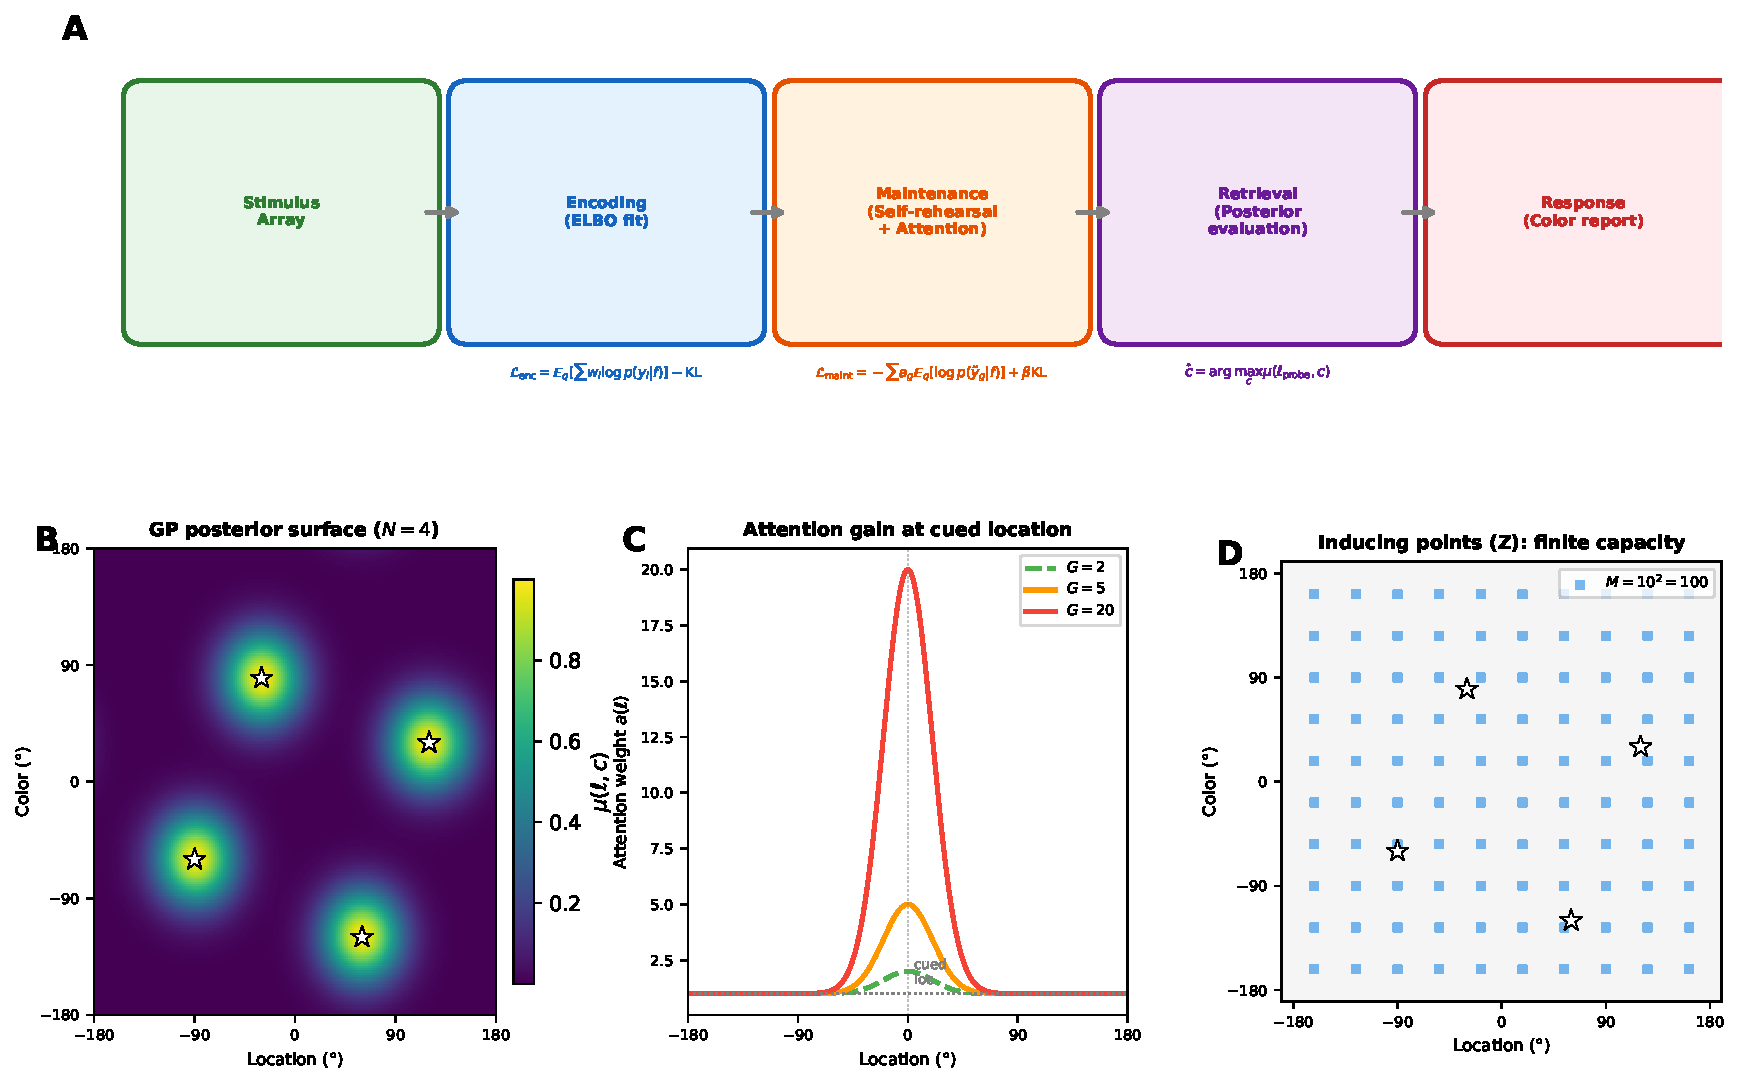
\includegraphics[width=\textwidth]{figures/fig1_schematic.pdf}
    \caption{\textbf{The MemGP framework.}
    \textbf{(A)} Computational pipeline. A stimulus array is encoded as noisy weighted observations; the GP posterior is fit via variational ELBO optimization. During maintenance, the posterior rehearses its own predictions under attention-weighted objectives with KL-divergence--driven forgetting. At retrieval, the posterior mean is evaluated at the probed location.
    \textbf{(B)} Example GP posterior surface for $N = 4$ items, showing localized peaks at each item's location--color coordinate.
    \textbf{(C)} Attention gain function: when a retrocue indicates a location, the maintenance ELBO weights are amplified near the cued location (gain $G$) while uncued locations remain at baseline.
    \textbf{(D)} The inducing-point grid ($\bZ$) defines the model's finite representational capacity; items compete for representation through these shared computational resources.}
    \label{fig:schematic}
\end{figure}

\begin{figure}[H]
    \centering
    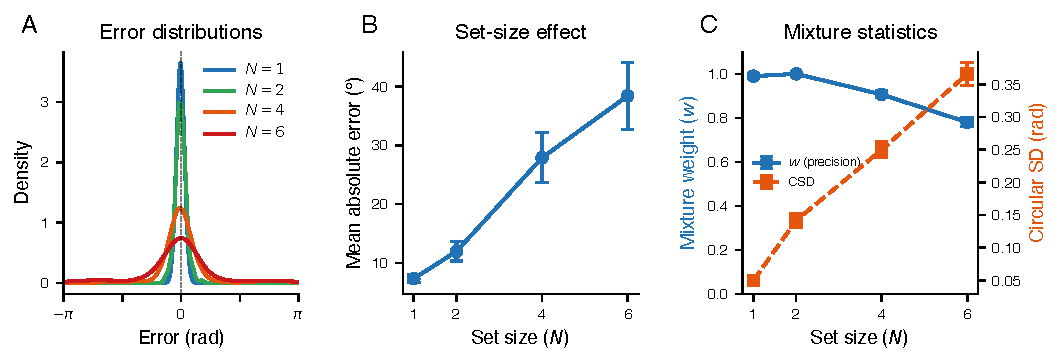
\includegraphics[width=\textwidth]{figures/fig2_set_size.pdf}
    \caption{\textbf{Set-size effects and model comparison.}
    \textbf{(A)} Kernel density estimates of signed recall errors across set sizes $N \in \{1, 2, 4, 6\}$, showing progressive broadening and flattening.
    \textbf{(B)} Mean absolute error increases monotonically with set size (error bars: $\pm 1$ SEM).
    \textbf{(C)} Mixture statistics (weight $w$ and circular SD) extracted from MemGP errors. $w$ declines with set size (apparent guessing) while CSD increases (declining precision).}
    \label{fig:setsize}
\end{figure}

\begin{figure}[H]
    \centering
    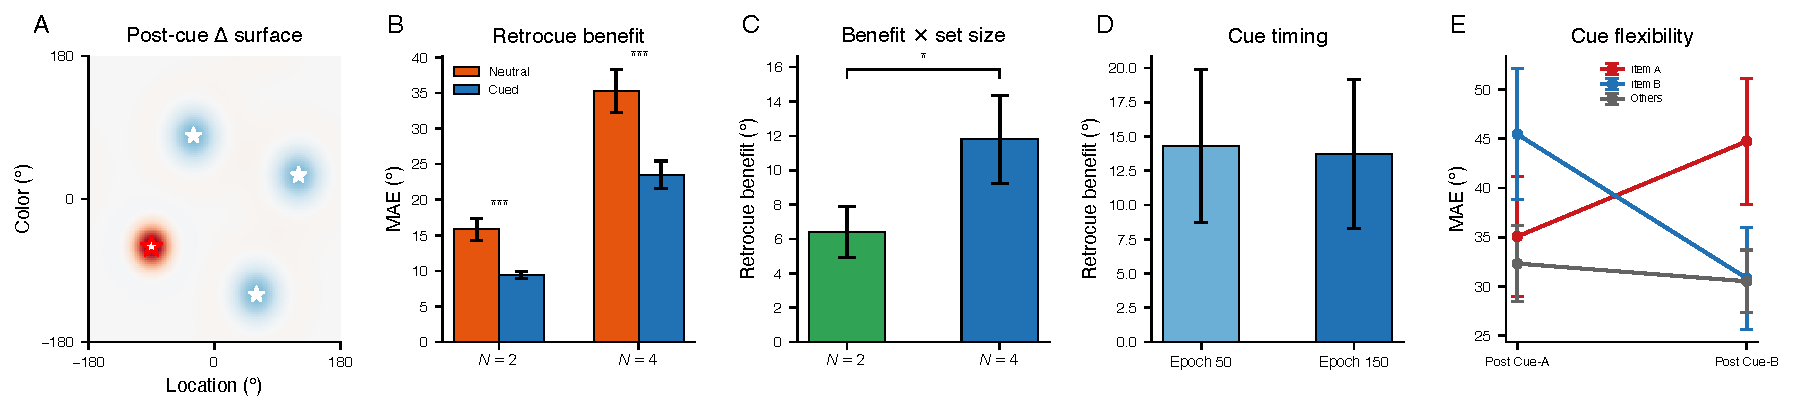
\includegraphics[width=\textwidth]{figures/fig3_retrocue.pdf}
    \caption{\textbf{Goal-driven maintenance and retrocue effects.}
    \textbf{(A)} Change in GP surface after retrocue: the cued item's peak is amplified (red/warm) while uncued items' peaks diminish (blue/cool).
    \textbf{(B)} Retrocue benefit: cued items are recalled with lower error than neutral (uncued) items.
    \textbf{(C)} The retrocue benefit increases with set size, consistent with greater competition at higher load.
    \textbf{(D)} Earlier cue onset produces a larger benefit.
    \textbf{(E)} Cue flexibility: when the cue shifts from item A to item B mid-maintenance, item B's accuracy improves while item A's degrades, demonstrating dynamic reallocation.}
    \label{fig:retrocue}
\end{figure}

\begin{figure}[H]
    \centering
    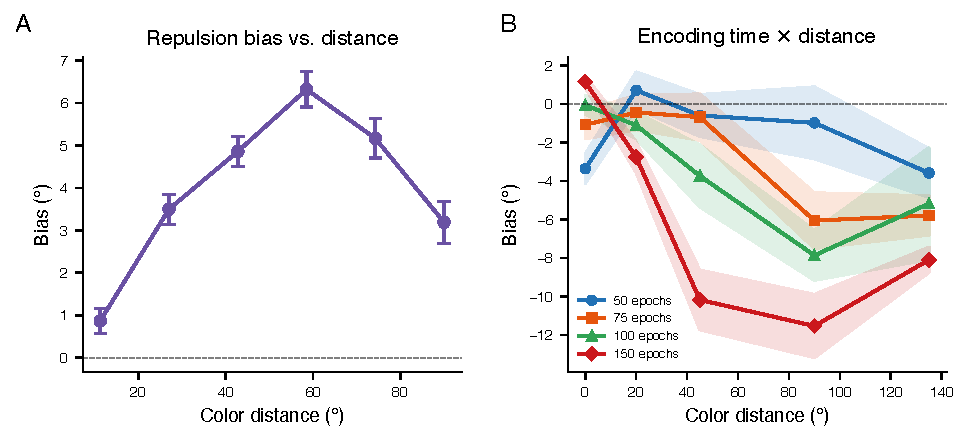
\includegraphics[width=\textwidth]{figures/fig4_bias.pdf}
    \caption{\textbf{Inter-item repulsion bias.}
    \textbf{(A)} Repulsion bias (negative = away from distractor) as a function of target--distractor color distance, showing the characteristic inverted-U pattern.
    \textbf{(B)} Encoding time $\times$ color distance interaction: shorter encoding (fewer epochs) produces stronger bias at small--medium distances, replicating the pattern reported by Chunharas et al.\ (2022). Shaded regions: $\pm 1$ SEM.}
    \label{fig:bias}
\end{figure}


% ╔═══════════════════════════════════════════════════════════════════════════╗
% ║  REFERENCES                                                               ║
% ╚═══════════════════════════════════════════════════════════════════════════╝
\bibliographystyle{unsrtnat}
\bibliography{../docs/references}


% ╔═══════════════════════════════════════════════════════════════════════════╗
% ║  SUPPLEMENTARY MATERIALS                                                  ║
% ╚═══════════════════════════════════════════════════════════════════════════╝
\clearpage
\appendix
\setcounter{figure}{0}
\setcounter{table}{0}
\renewcommand{\thefigure}{S\arabic{figure}}
\renewcommand{\thetable}{S\arabic{table}}

\section*{Supplementary Materials}

\subsection*{S1. Mathematical formulation}

\subsubsection*{S1.1 Gaussian process prior}

We model the latent memory function $f: \mathcal{X} \to \R$ where $\mathcal{X} = [-180, 180)^2$ is the circular location--color space. The GP prior is:
\[
f \sim \GP\bigl(m_0, \, k(\bx, \bx')\bigr)
\]
with constant mean $m_0$ and covariance:
\[
k(\bx, \bx') = \sigma^2_f \cdot k_{\mathrm{per}}(\ell, \ell'; \lambda_\ell, P) \cdot k_{\mathrm{per}}(c, c'; \lambda_c, P)
\]
where the periodic kernel is:
\[
k_{\mathrm{per}}(x, x'; \lambda, P) = \exp\!\left(-\frac{2 \sin^2(\pi |x - x'| / P)}{\lambda^2}\right)
\]
with period $P = 360^\circ$ for both dimensions. The output scale $\sigma^2_f$ is learned as part of a \texttt{ScaleKernel} wrapper.

\subsubsection*{S1.2 Sparse variational approximation}

We approximate the true posterior $p(f \mid \mathcal{D})$ using $M$ inducing points $\bZ \in \R^{M \times 2}$ with inducing function values $\bu = f(\bZ)$. The variational distribution is:
\[
q(\bu) = \mathcal{N}(\bu; \, \bm, \, \mathbf{S})
\]
with $\mathbf{S}$ parameterized via its Cholesky factor (CholeskyVariationalDistribution). The conditional posterior at any test point is obtained via the standard SVGP predictive equations:
\[
q(f(\bx^*)) = \mathcal{N}\!\left(
    \mathbf{k}_*^\top \mathbf{K}_{ZZ}^{-1} \bm, \;
    k_{**} - \mathbf{k}_*^\top \mathbf{K}_{ZZ}^{-1}(\mathbf{K}_{ZZ} - \mathbf{S})\mathbf{K}_{ZZ}^{-1} \mathbf{k}_*
\right)
\]
where $\mathbf{k}_* = k(\bZ, \bx^*)$ and $\mathbf{K}_{ZZ} = k(\bZ, \bZ)$.

Inducing points are initialized on a regular $m \times m$ grid ($m = 10$ by default, $M = 100$) with centers offset by half the bin width to ensure uniform coverage. They are optionally learned during optimization (\texttt{learn\_inducing\_locations = True}).

\subsubsection*{S1.3 Encoding objective}

Given $N$ items $\{(\ell_i, c_i)\}_{i=1}^N$, each generates $n_{\mathrm{obs}}$ noisy observations $\bx_{ij} = (\ell_i + \epsilon_{\ell}, c_i + \epsilon_c)$ with $\epsilon_\ell \sim \mathcal{N}(0, \sigma_\ell^2)$, $\epsilon_c \sim \mathcal{N}(0, \sigma_c^2)$, wrapped to $[-180, 180)$. Importance weights are:
\[
w_{ij} = \exp\!\left(-\frac{d_\ell(\bx_{ij}, \bx_i^{\mathrm{enc}})^2}{2\sigma_\ell^2}\right) \cdot \exp\!\left(-\frac{d_c(\bx_{ij}, \bx_i^{\mathrm{enc}})^2}{2\sigma_c^2}\right)
\]
where $d_\ell, d_c$ are circular distances and $\bx_i^{\mathrm{enc}}$ is the (possibly noise-shifted) encoded center.

The encoding ELBO is maximized using Adam with learning rate $\eta_{\mathrm{enc}} = 0.05$ for $T_{\mathrm{enc}} = 100$ epochs. The Gaussian likelihood has fixed noise variance $\sigma_n^2 = 10^{-6}$ (not learned).

\subsubsection*{S1.4 Maintenance objective}

A dense maintenance grid $\mathcal{G}$ of $G \times G$ points ($G = 30$ by default, $|\mathcal{G}| = 900$) covers the torus uniformly. Pseudo-targets are frozen as the posterior mean at the end of encoding:
\[
\tilde{y}_g = \E_{q(f)}[f(\bx_g)] \quad \forall g \in \mathcal{G}
\]

The maintenance objective (Eq.~\ref{eq:elbo_maint}) is optimized with Adam at learning rate $\eta_{\mathrm{maint}} = 0.01$--$0.015$ for $T_{\mathrm{maint}} = 100$--$200$ epochs. The KL coefficient $\beta$ controls forgetting speed: $\beta = 1$ (standard) or $\beta = 5$ (enhanced retrocue sensitivity). Before cue onset (epoch $t_{\mathrm{cue}}$), attention weights are uniform ($a_g = 1$). After cue onset, the spatial gain function (Eq.~\ref{eq:attention}) with parameters $G$ (attended gain) and $\sigma_s$ (spatial width) is applied.

\subsubsection*{S1.5 Retrieval}

\textbf{MAP retrieval:} $\hat{c} = \arg\max_{c \in \{-180, \ldots, 179\}} \mu(\ell_{\mathrm{probe}}, c)$ where $\mu$ is the posterior mean evaluated at 360 evenly spaced color values.

\textbf{Divisive normalization (bias experiments):} The 2D posterior surface is evaluated, shifted nonnegative, and a spatial Gaussian pool is computed at each color value:
\[
\mathrm{pool}(c) = \sum_{\ell'} w_{\mathrm{sp}}(\ell') \cdot f^+(\ell', c)
\]
with spatial weights $w_{\mathrm{sp}}(\ell') \propto \exp(-d(\ell', \ell_{\mathrm{probe}})^2 / 2\sigma_{\mathrm{pool}}^2)$, followed by circular smoothing in color space. The normalized response is:
\[
r(c) = \frac{f^+(\ell_{\mathrm{probe}}, c)}{\sigma_b \cdot \max_c f^+(\ell_{\mathrm{probe}}, c) + \mathrm{pool}(c)}
\]
where $\sigma_b$ is the baseline fraction.


\subsection*{S2. Simulation parameters}

\begin{table}[H]
\centering
\caption{Configuration parameters across experiments.}
\label{tab:params}
\small
\begin{tabular}{lccc}
\toprule
\textbf{Parameter} & \textbf{Set-size} & \textbf{Retrocue} & \textbf{Bias} \\
\midrule
$n_{\mathrm{obs}}$ per item & 1000 & 1000 & 1000 \\
$\sigma_\ell$ (loc sampling noise) & $20^\circ$ & $20^\circ$ & $20^\circ$ \\
$\sigma_c$ (color sampling noise) & $20^\circ$ & $20^\circ$ & $20^\circ$ \\
Loc encoding noise & $0^\circ$ & $0^\circ$ & $20^\circ$ \\
$m$ (inducing grid side) & 10 & 10 & 10 \\
$G_{\mathrm{maint}}$ (maint grid side) & 30 & 30 & 30 \\
$\lambda_\ell$ (loc lengthscale) & 10.0 & 10.0 & 10.0 \\
$\lambda_c$ (color lengthscale) & 10.0 & 10.0 & 10.0 \\
$\sigma_n^2$ (likelihood noise) & $10^{-6}$ & $10^{-4}$ & $10^{-6}$ \\
$T_{\mathrm{enc}}$ (encoding epochs) & 100 & 100 & varies \\
$T_{\mathrm{maint}}$ (maintenance epochs) & 100 & 200 & 100 \\
$\eta_{\mathrm{enc}}$ (encoding LR) & 0.05 & 0.05 & 0.05 \\
$\eta_{\mathrm{maint}}$ (maintenance LR) & 0.01 & 0.015 & 0.01 \\
$\beta$ (KL weight) & 1 & 5 & 1 \\
$\sigma_s$ (attention spatial width) & $20^\circ$ & $20^\circ$ & $20^\circ$ \\
$G$ (attended gain) & 2.0 & 20.0 & 2.0 \\
Loc pool width (normalization) & --- & --- & $60^\circ$ \\
Color pool width (normalization) & --- & --- & $5^\circ$ \\
Baseline fraction ($\sigma_b$) & --- & --- & 0.5 \\
\bottomrule
\end{tabular}
\end{table}


\subsection*{S3. Information-theoretic model comparison}

For each benchmark model $\mathcal{M}$ with $k$ free parameters fit by MLE to $n$ total observations, we computed:
\begin{align}
    \mathrm{AIC} &= 2k - 2\ln \hat{L} \\
    \mathrm{BIC} &= k \ln n - 2\ln \hat{L} \\
    \mathrm{AICc} &= \mathrm{AIC} + \frac{2k(k+1)}{n - k - 1}
\end{align}
where $\hat{L}$ is the maximized likelihood. Models with lower AIC/BIC are preferred. Parameter counts: IL ($k=3$: $K, \kappa_{\mathrm{mem}}, \kappa_r$), SA ($k=3$: $K, J_1, \kappa_r$), EP ($k=3$: $J_1, \alpha, \kappa_r$), VP ($k=4$: $\bar{J}_1, \alpha, \tau, \kappa_r$).


\subsection*{S4. Parameter sensitivity analysis}

To assess the robustness of MemGP's qualitative predictions, we systematically varied three key parameters while holding others at default values (Supplementary Fig.~S2):

\begin{itemize}
\item \textbf{Inducing grid size} ($m \in \{6, 10, 16\}$, corresponding to $M \in \{36, 100, 256\}$): Larger grids reduce errors at all set sizes, but the qualitative pattern of increasing error with $N$ is preserved across all grid sizes.
\item \textbf{KL weight} ($\beta \in \{0.1, 1, 5\}$): Higher $\beta$ accelerates forgetting, increasing errors uniformly, but the set-size gradient is maintained. The retrocue benefit increases with $\beta$, as stronger forgetting pressure makes attentional support more valuable.
\item \textbf{Kernel lengthscale} ($\lambda \in \{5, 10, 20\}$): Shorter lengthscales produce sharper peaks and lower errors for small $N$, but capacity-driven degradation at large $N$ remains qualitatively consistent.
\end{itemize}

\begin{figure}[H]
    \centering
    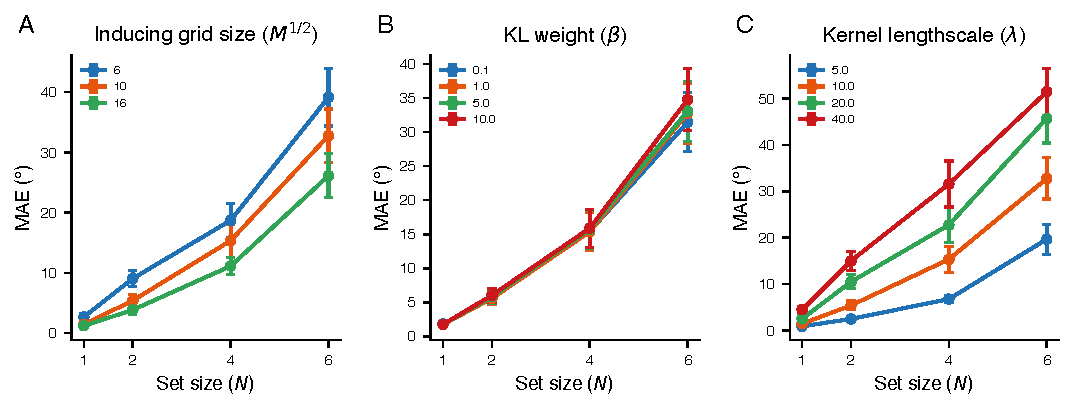
\includegraphics[width=\textwidth]{figures/fig_param_sensitivity.pdf}
    \caption{\textbf{Supplementary Figure S2: Parameter sensitivity analysis.}
    Mean absolute error vs.\ set size under systematic variation of three key model parameters.
    \textbf{(A)}~Inducing grid size $m \in \{6, 10, 16\}$ ($M = m^2$ inducing points): larger grids reduce error at all set sizes, but the monotonic set-size gradient is preserved.
    \textbf{(B)}~KL weight $\beta \in \{0.1, 1, 5\}$: higher $\beta$ accelerates forgetting and increases error, while the qualitative set-size pattern remains stable.
    \textbf{(C)}~Kernel lengthscale $\lambda \in \{5, 10, 20\}$: shorter lengthscales yield sharper item peaks and lower error for small $N$, but all values produce increasing error with set size.}
    \label{fig:param_sensitivity}
\end{figure}

\begin{figure}[H]
    \centering
    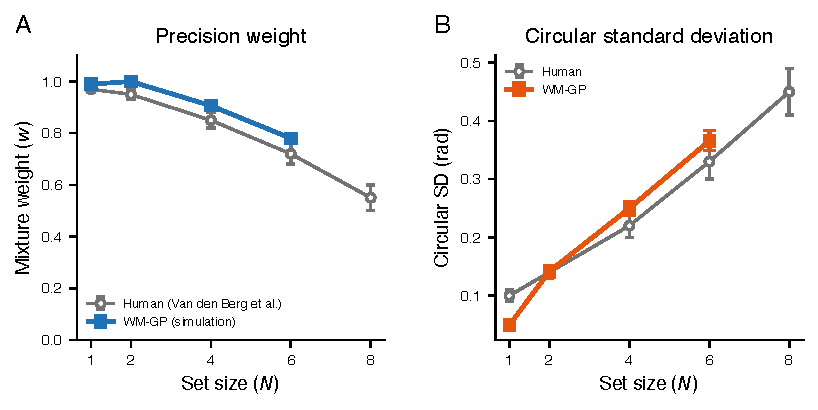
\includegraphics[width=\textwidth]{figures/fig_human_overlay_setsize.pdf}
    \caption{\textbf{Supplementary Figure S1: Comparison with human data.}
    MemGP mixture statistics ($w$, CSD) overlaid with approximate human data from Van den Berg et al.\ (2012). The model's emergent error profile falls within the empirical range.}
    \label{fig:human_overlay}
\end{figure}


\end{document}
